\newcommand{\triabc}{{\triangle ABC}}
\newcommand{\squarewxyz}{\square{WXYZ}}
\section{Proofs with Geometry}

% distributing property
\begin{theorem}
    $\times$ distributes over $+$. That is, for $a, b, c \in \reals$,
    $a(b+c) = ab + bc = (b+c)a$.
\end{theorem}

\begin{corollary} \label{direct: cor: foil}
    Let $a, b, c, d \in \reals$. Then 
    $(a + b)(c + d) = ac + ad + bc + bd$.
\end{corollary}
\begin{proof}
    See questions.
\end{proof}


% Pythagoras' theorem
\begin{theorem} (Pythagoras' Theorem)
    Given any right-angled triangle $\triabc$ where $AC$ is 
    the hypotenuse, we have:
    $$|AB|^2 + |BC|^2 = |AC|^2.$$ 
\end{theorem}
\begin{proof}
    Let $\triabc$ be an arbitrary right-angled triangle, and let 
    $a \equiv |AB|$, $b \equiv |BC|$ and $c \equiv |AC|$ We
    construct the square $\square WXYZ$ by connecting four similar triangles
    base side to hight side as in Figure \ref{direct: fig: pyth}.
    % TODO: question: verify that is a square.

    The area of $WXYZ$, $A_{WXYZ}$, is equal to $c^2$ because 
    $|WX| = |AC|$. However, we can compute its $A_{WXYZ}$ a different way.
    By our  construction, we find that $A_{WXYZ}$ is equal to the four
    triangle areas plus the smaller square in the middle. The side of the
    square is equal to $|BC| - |AC| = b - a$. So, at last we get:  
    \begin{align}
        A_{WXYZ}   &= 4(ba / 2) + (b-a)^2 & \justify{from above} \\
                   &= 2ba + (b^2 - 2ba + a^2)
                     & \justify{by Corollary \ref{direct: cor: foil}} \\
                   &= b^2 + a^2
    \end{align}
    So, $c^2 = A_{WXYZ} = b^2 + a^2$ and so our result follows by transitivity.
\end{proof}

\begin{figure}
    \begin{subfigure}{0.4\linewidth}
        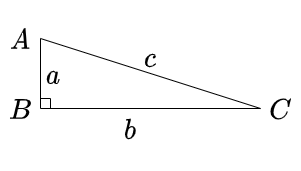
\includegraphics[width=\linewidth]
        {src/direct_src/pythagorean-triangle.png}
        \caption{An arbitrary right angle $\triabc$ 
        with side lengths $|AB| = a, |BC| = b, |AC| = c.$}
    \end{subfigure}
    \begin{subfigure}{0.5\linewidth}
        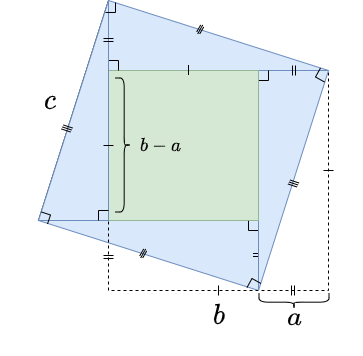
\includegraphics[width=\linewidth]
        {src/direct_src/pythagorean-final.png}
        \caption{Square $A_{WXYZ}$ constructed from $\triabc$.}
    \end{subfigure}
    \caption{Crucial Shapes of the Pythagorean Theorem proof.}
     \label{direct: fig: pyth}
\end{figure}

With this powerful tool in hand, we prove the more general case:
\begin{theorem} [Cosine Law]
    Given any triangle $\triangle ABC$, denote the longest side as
    $AC$ and denote the angle that the line segment $AB$ makes with $BC$. 
    Then $$|AC|^2 = |AB|^2 + |BC|^2 - |AB||BC| \cos(\theta).$$
\end{theorem}


And so the cosine law leads us to this result.
\begin{corollary}
    Let $a, b, c \in \reals$ be lengths such that $a \leq b \leq c$.
    Then, a triangle can be formed with lenghts $a, b, c$ iff $a-b < c < a+b$. 
\end{corollary}
\begin{proof} \.
    [$\implies$] Suppose that $\triabc$ is a triangle, where $AC$ is the
    longest side with length $c$. Then, $\triabc$ satisfies the cosine
    law. Since $-1 \leq cos(\theta) \leq 1$, we get:
    \begin{align}
        c^2 &= a^2 + b^2 - 2ab\cos(\theta) \\
            &> a^2 + b^2 - 2ab, & \justify{When $\theta = 0$} \\
            &= (a - b)^2, & \justify{By Corollary \ref{direct: cor: foil}}
    \end{align}
    and
    \begin{align}
        c^2 &< a^2 + b^2 + 2ab, & \justify{When $\theta = \pi$} \\
            &= (a + b)^2.
    \end{align}
    
    Taking square roots of the inequalities, we achieve our desired result.

    [$\impliedby$] Suppose that $a, b, c; a < b < c$ are positive
    lengths such that $|b - a| < c < a + b$.  We wish to prove
    that we can make a triangle out of these lengths.

    From the proof of the opposide direction, it is easy to see that 
    $c^2 = a^2 + b^2 - 2ab\cos(\theta)$ for some $\theta \in (0, \pi)$.
    Construct a triangle $\triabc$ such that $AB$ is parallel on the
    x-axis with length $a$, and $BC$ extends from $AB$'s left-most point,
    turning $\pi$ radians  counter-clockwise as in Figure %TODO 

    Using Pythagoras' Theorem, we calculate $|AC|^2$:
    \begin{align}
        &|AC|^2 \\
        &= (a + b\sin(\theta - \pi/2))^2 - (b\cos(\theta - \pi/2))^2 \\
        &= a^2 - 2ab\cos(\theta) + b^2\cos^2(\theta) + b^2\sin^2(\theta)
         & \justify{Translating $\sin, \cos$ right} \\
        &= a^2 - 2ab\cos(\theta) + b^2 (\sin^2(\theta) + \cos^2(\theta)) \\
        &= a^2 + b^2 - 2ab\cos(\theta) \\
        &= c^2
    \end{align}
    So $|AC| = c$, as wanted.
\end{proof}

